\documentclass{article}
\usepackage[margin=1.0in]{geometry}
\usepackage{amsmath, amssymb, mathrsfs}
\usepackage[english]{babel}
\usepackage{graphicx}
\usepackage{enumerate}
\usepackage{listings}
\usepackage{tikz}
\usepackage{pgfplots}
\renewcommand{\vec}[1]{\mathbf{#1}}
\newcommand{\floor}[1]{\left\lfloor #1 \right\rfloor}
\newcommand{\ceil}[1]{\left\lceil #1 \right\rceil}
\DeclareMathOperator{\Tr}{Tr}

\title{Machine Learning from Data Assignment 6}
\author{Greg Stewart}
\date{\today}

\begin{document}

\maketitle

\subsection*{Exercise 3.4}

\textit{Consider noisy target $y=w^{*T}x + \epsilon$ for generating data, where $\epsilon$ is a
noise term with zero mean and $\sigma^2$ variance, independently generated for every example
$\vec{x},y$. Expected error of best possible linear fit to the target is $\sigma^2$.
For the data $D$ denote the noise in $y_n$ as $\epsilon_n$ and let $\vec{\epsilon} = [\epsilon_1,
\epsilon_2, \dots, \epsilon_N]^T$, and assume $X^TX$ is invertible. Follow the steps to show the expected in sample error of linear regression w.r.t. $D$ is given by}

$$\mathbb{E}_D[E_{in}(\vec{w}_{lin})] = \sigma^2 (1 - \frac{d+1}{N}).$$

\begin{enumerate}[(a)]
  \item \textit{Show that the in sample estimate of $\vec{y}$ is given by
    $\hat{\vec{y}} = X\vec{w}^* + H\epsilon$.}

    Since $\hat{\vec{y}} = H\vec{y}$, we can use the definition of $H$ and of $\vec{y}$ to 
    arrive at this result.

    \begin{align*}
      \hat{\vec{y}} &= [X(X^TX)^{-1}X^T](X\vec{w}^* + \vec{\epsilon}) \\
      &= X[(x^TX)^{-1}(X^TX)]\vec{w}^* + H\vec{\epsilon} \\
      &= X\vec{w}^* + H\vec{\epsilon} \\
    \end{align*}

  \item \textit{Show the in sample error vector $\hat{\vec{y}} - \vec{y}$ can be expressed by a
    matrix times $\epsilon$. What is the matrix?}

    \begin{align*}
      \hat{\vec{y}} - \vec{y} &= X\vec{w}^* + H\vec{\epsilon} - (X\vec{w}^* + \vec{\epsilon}) \\
      &= H\vec{\epsilon} - \vec{\epsilon} = (H - I)\vec{\epsilon}
    \end{align*}

    So obviously the matrix in question is $(H - I)$.

  \item \textit{Express $E_{in}(\vec{w}_{lin})$ in terms of $\vec{\epsilon}$ using (b), and
    simplify the expression using Exercise 3.3(c).}

    \begin{align*}
      E_{in}(\vec{w}_{lin}) &= \frac{1}{N} ||\hat{\vec{y}} - \vec{y}||^2 \\
      &= \frac{1}{N}[\vec{\epsilon}^T(H-I)^T][(H-I)\vec{\epsilon}] \\
      &= \frac{1}{N}\vec{\epsilon}^T(H-I)^2\vec{\epsilon} \\
      &= \frac{1}{N}\vec{\epsilon}^T(I-H)\vec{\epsilon} \\
      &= \frac{1}{N}(\vec{\epsilon}^T\vec{\epsilon} - \vec{\epsilon}^TH\vec{\epsilon})
    \end{align*}

    where we have used the fact that $(I-H)^k = (I-H)$.

  \item \textit{Prove the original equality we sought.}

    \begin{align*}
      \mathbb{E}_D[E_{in}] &= \mathbb{E}_D[\frac{1}{N}\epsilon^T\epsilon] - 
          \mathbb{E}_D[\frac{1}{N}\epsilon^TH\epsilon] \\
      &= \frac{N\sigma^2}{N} - \frac{1}{N}\mathbb{E}_D[\sum_iH_{ii}\epsilon_i^2]
          - \frac{1}{N}\mathbb{E}_D[\sum_{i,j}H_{ij}\epsilon_i\epsilon_j] \\
      &= \sigma^2 - \frac{1}{N}\Tr{H}\epsilon_i^2 - \frac{1}{N}(0) \\
      &= \sigma^2 - \frac{1}{N}(d+1) \\
      &= \sigma^2(1 - \frac{d+1}{N})
    \end{align*}


  \item

    As the noise term is a random variable and likely follows a normal distribution, the 
    expectation of the noise term is again 0. Since the rest of the test data comes from the
    same target function, we end up with the same expected error. That is,

    $$\mathbb{E}_{D,\epsilon'}[E_{test}(\vec{w}_{lin})] = \sigma^2(1 + \frac{d+1}{N})$$

\end{enumerate}



\subsection*{Problem 3.1}

\textit{Use 2000 uniformly generated samples for the two semicircle region for this problem.}

\begin{enumerate}[(a)]
  \item \textit{Run the PLA starting from $\vec{w} = \vec{0}$ until convergence, and plot.}

    \begin{center}
      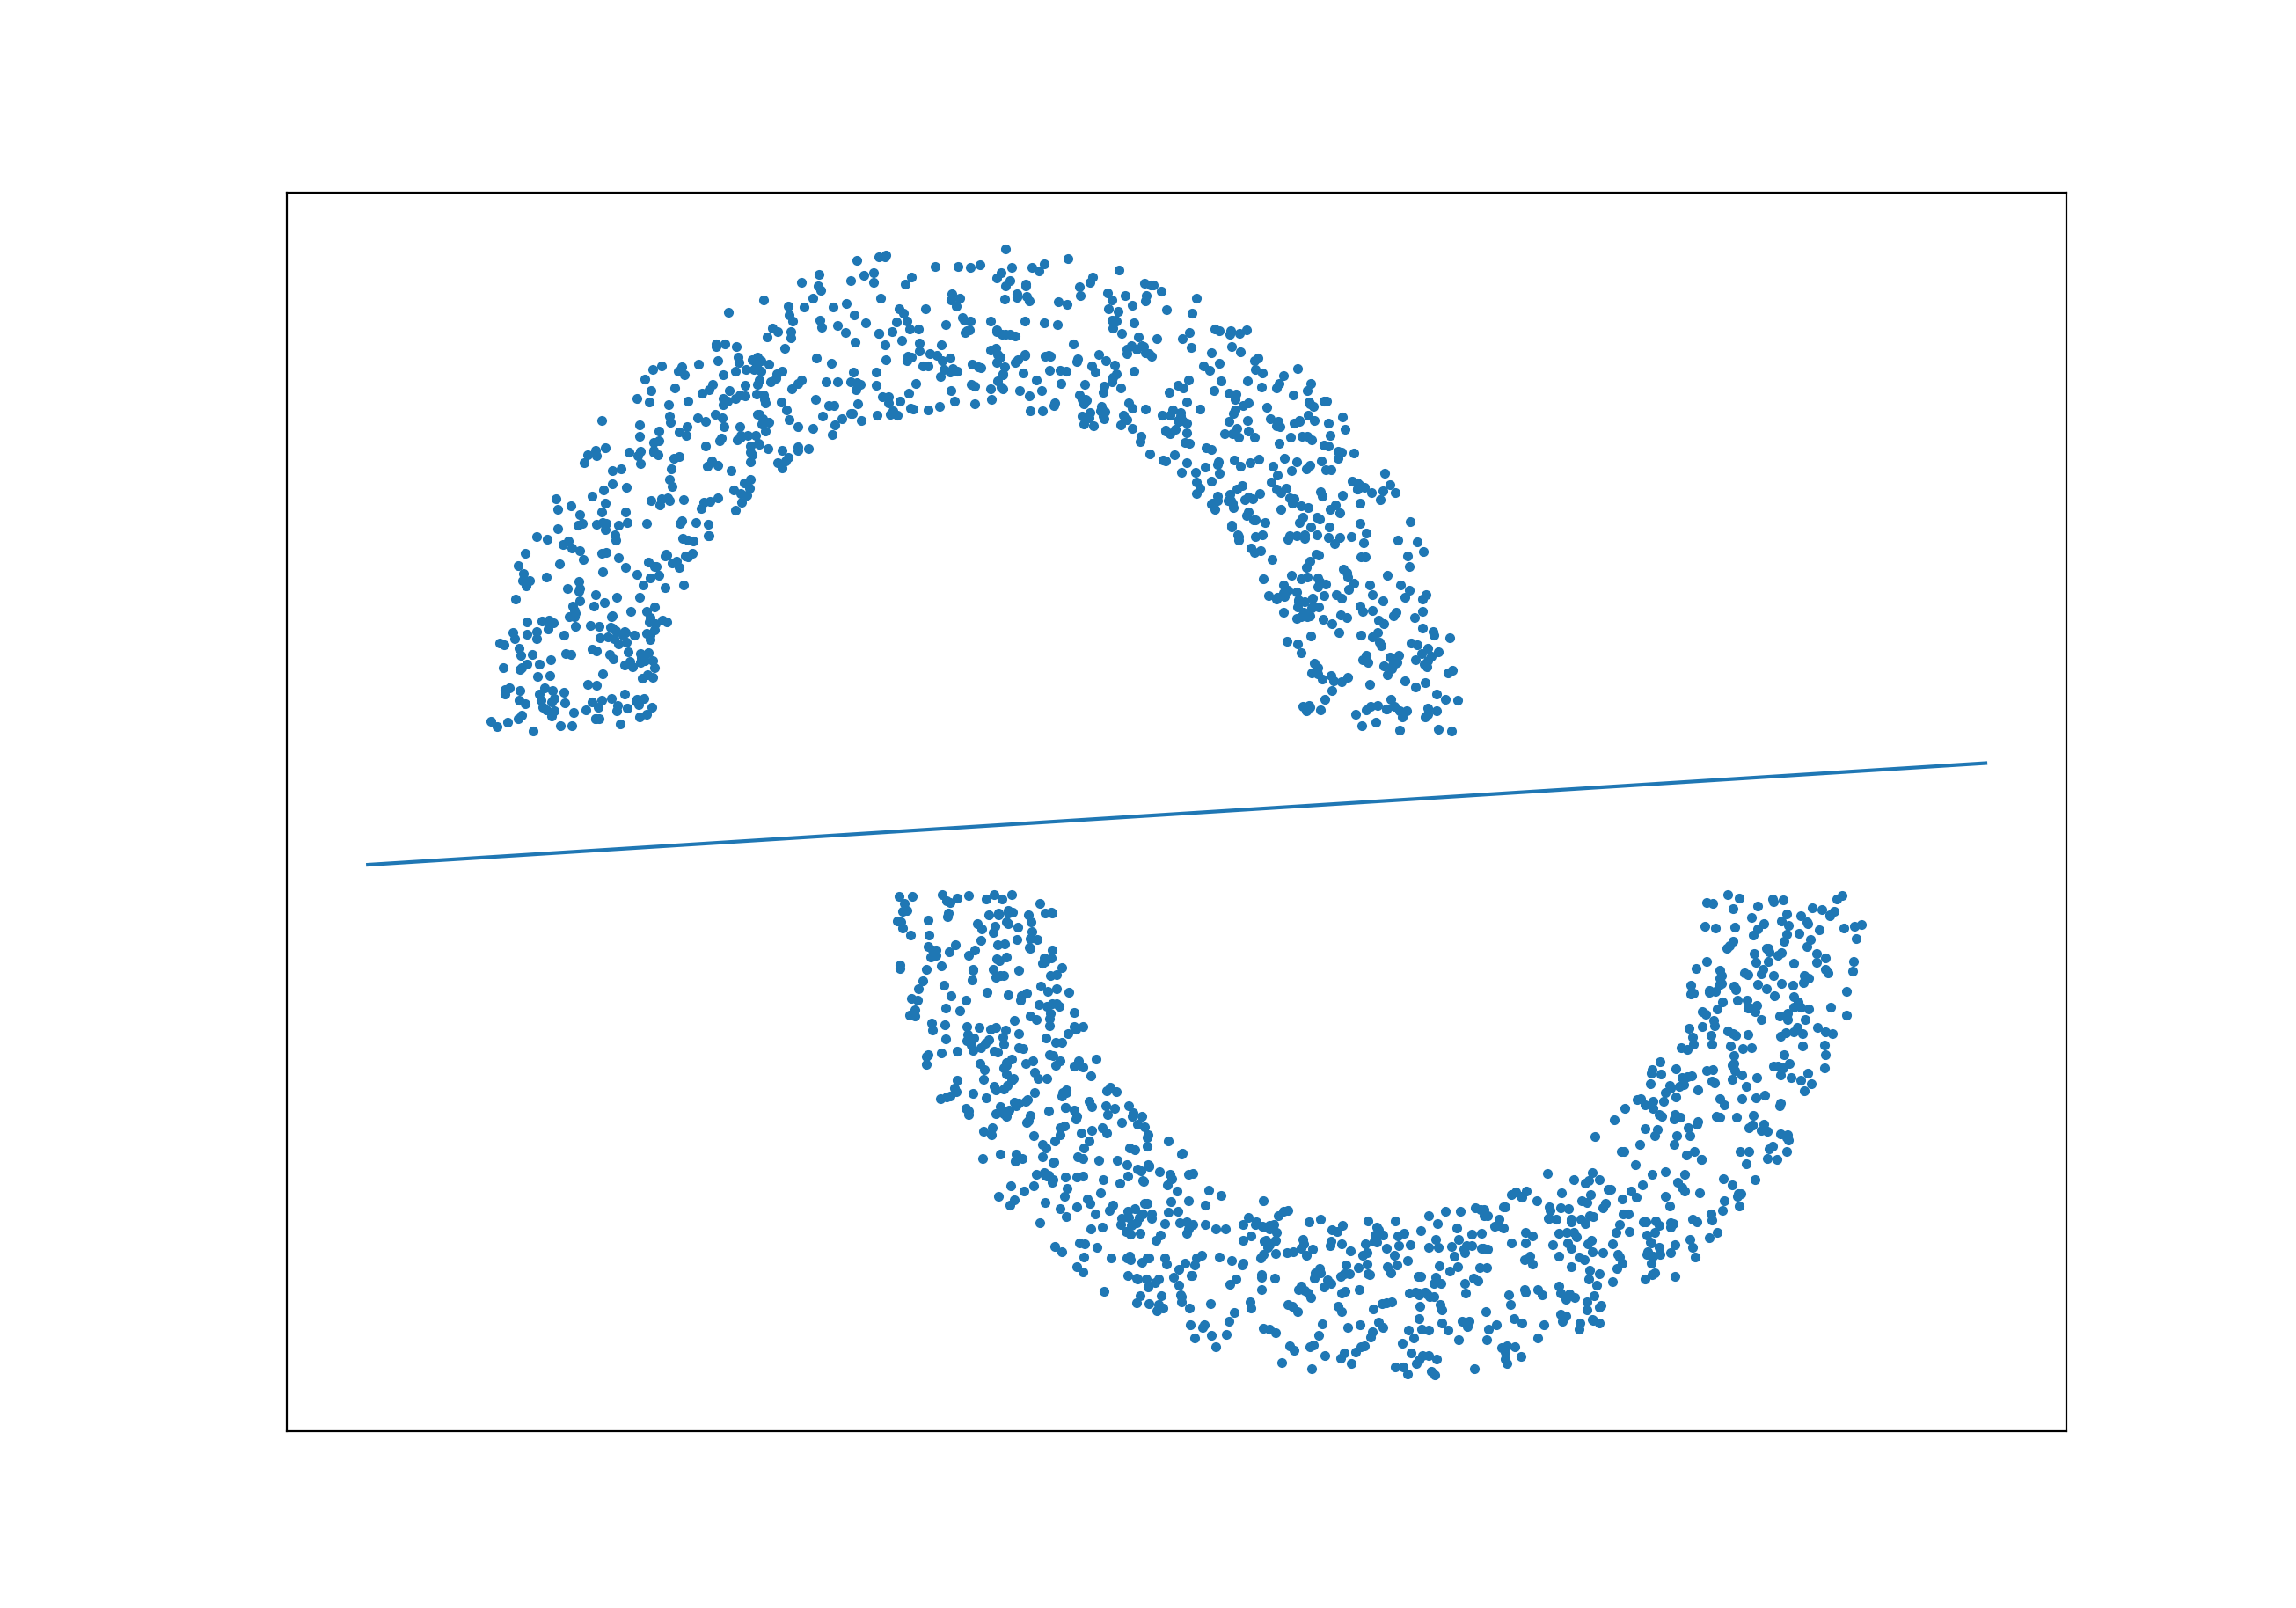
\includegraphics[width=\textwidth]{31a.png}
    \end{center}

  \item \textit{Repeat (a) using linear regression and explain.}

    \begin{center}
      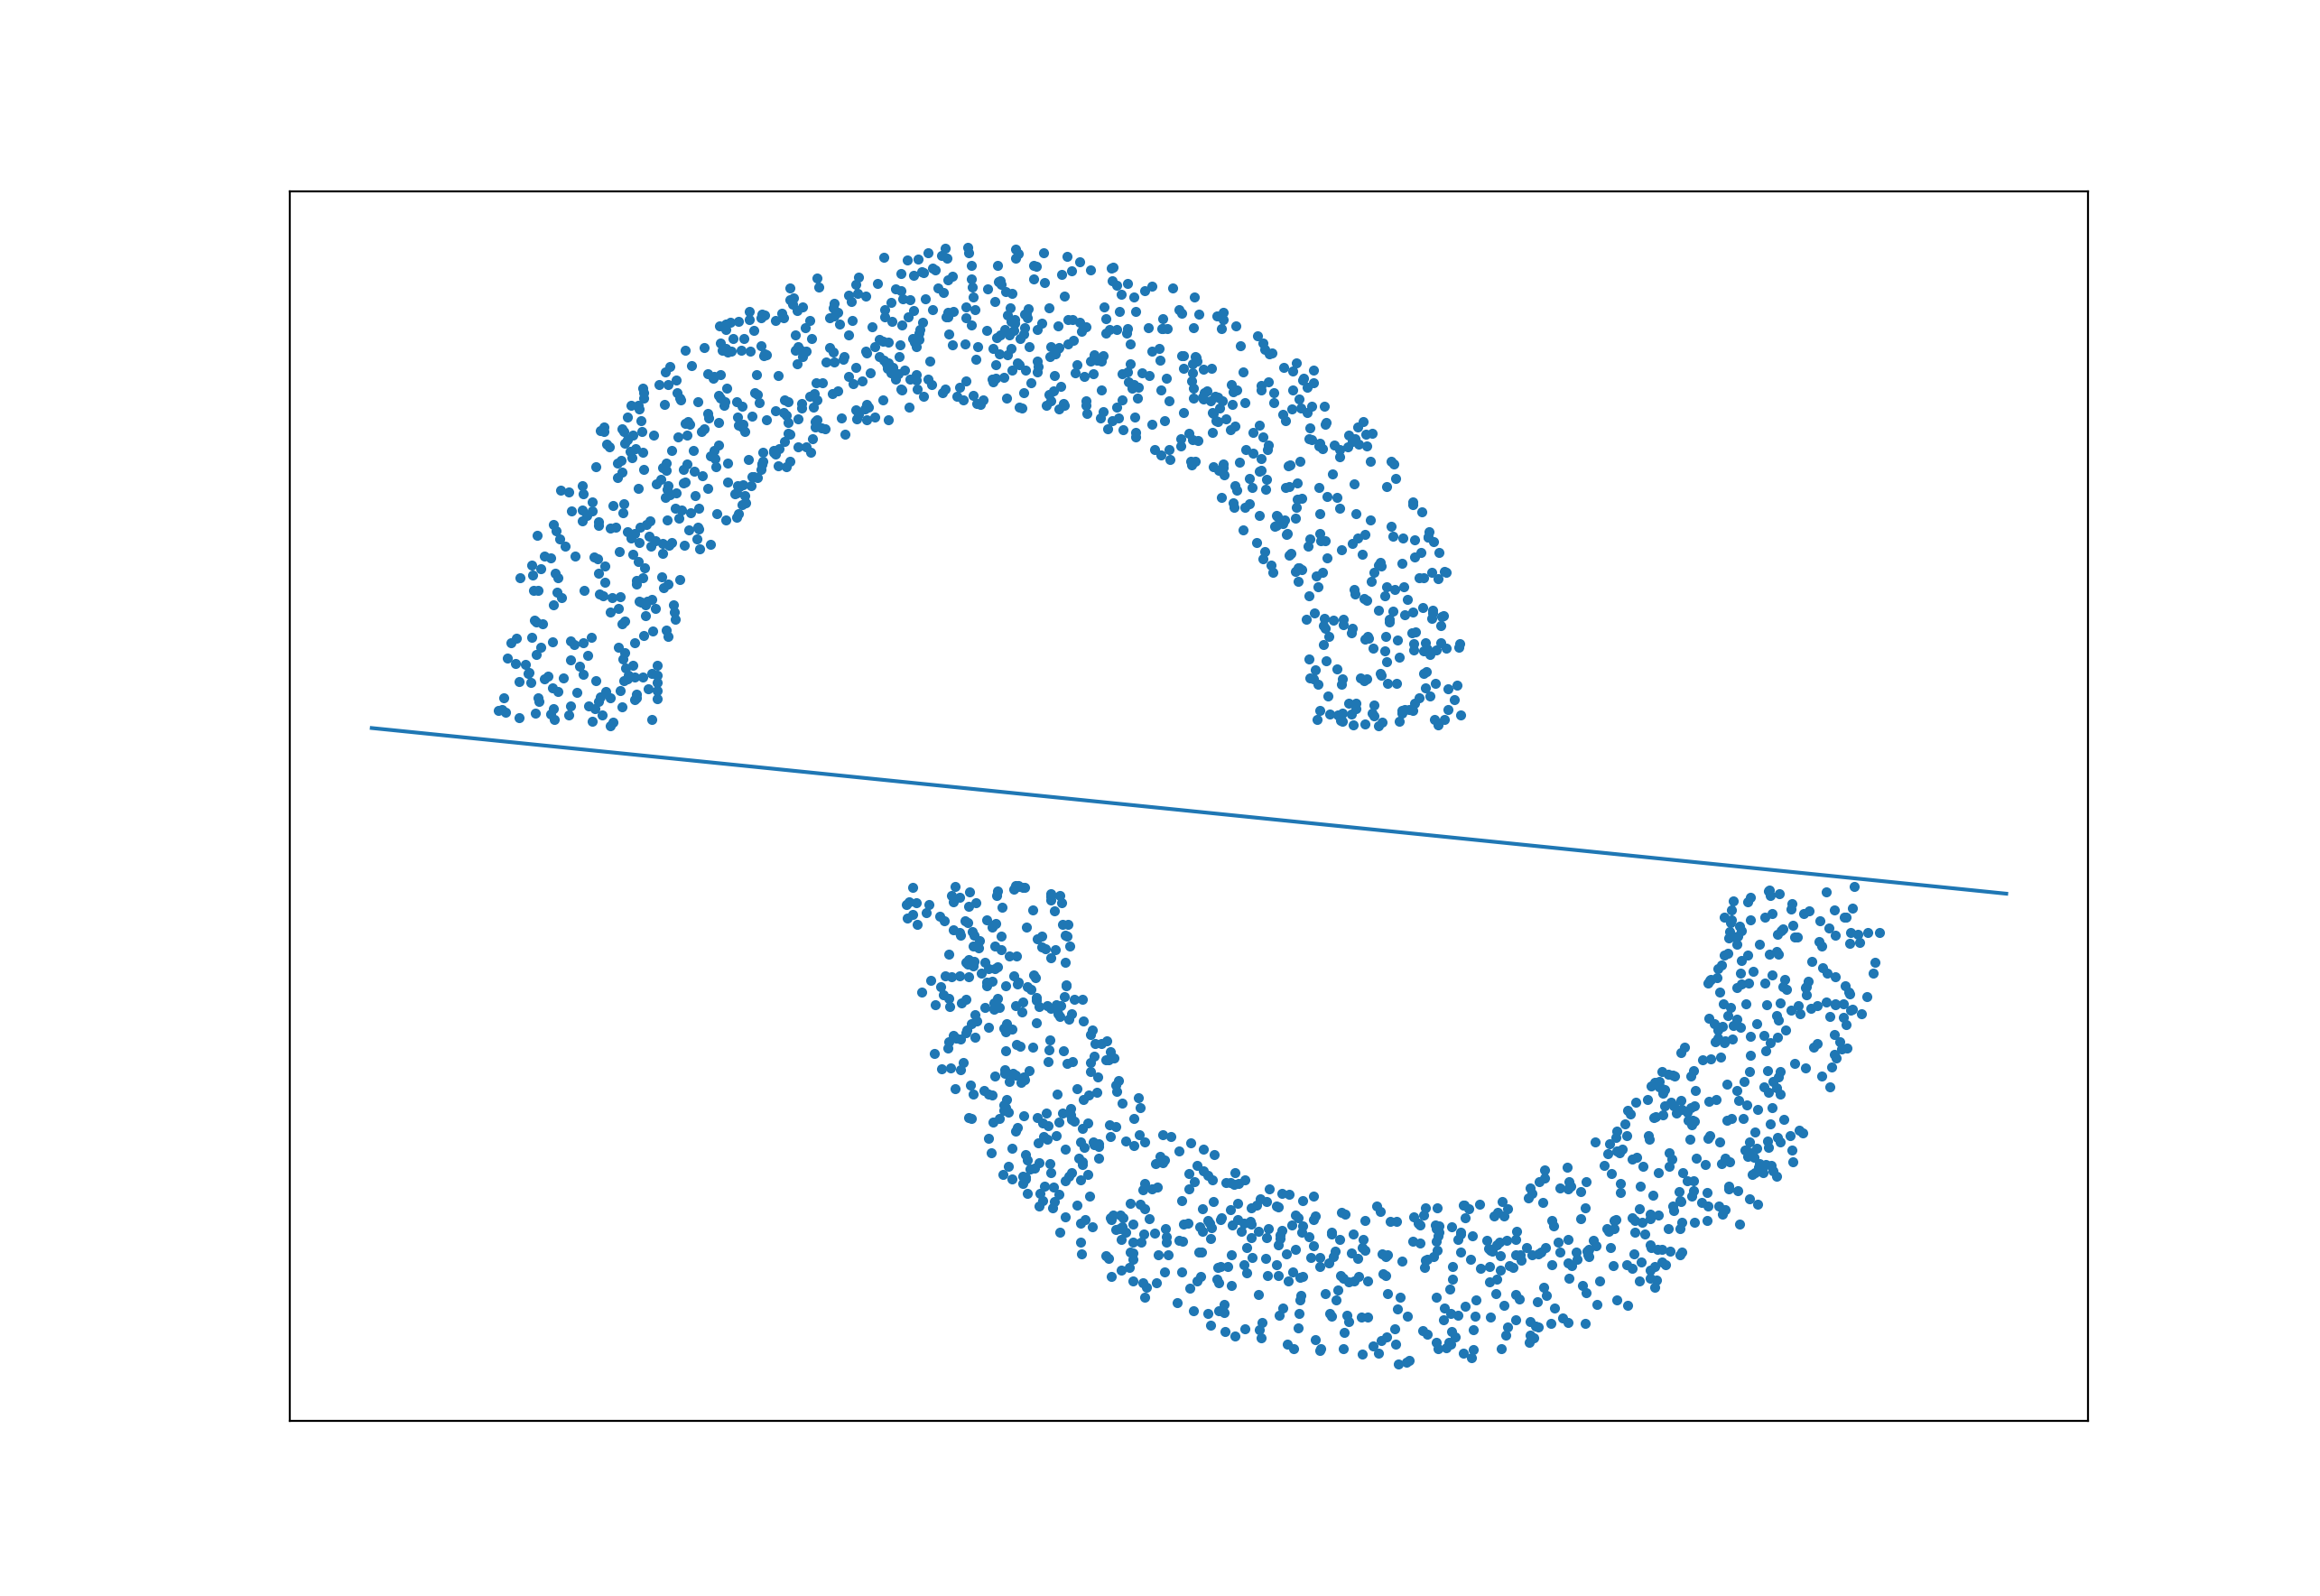
\includegraphics[width=\textwidth]{31b.png}
    \end{center}

    Since the data is linearly separable, linear regression easily separates the data, just as
    PLA was able to do. However, this is closer to an "optimum" linear hypothesis, which explains
    the difference in slope. This regression produced a negative slope, corresponding to the
    densities of data points. PLA was not able to do this because it simply adjusts based on what
    data is misclassified on each iteration.

\end{enumerate}



\subsection*{Problem 3.2}

\textit{Vary the separation and plot sep vs. the number of iterations of PLA. Explain.}

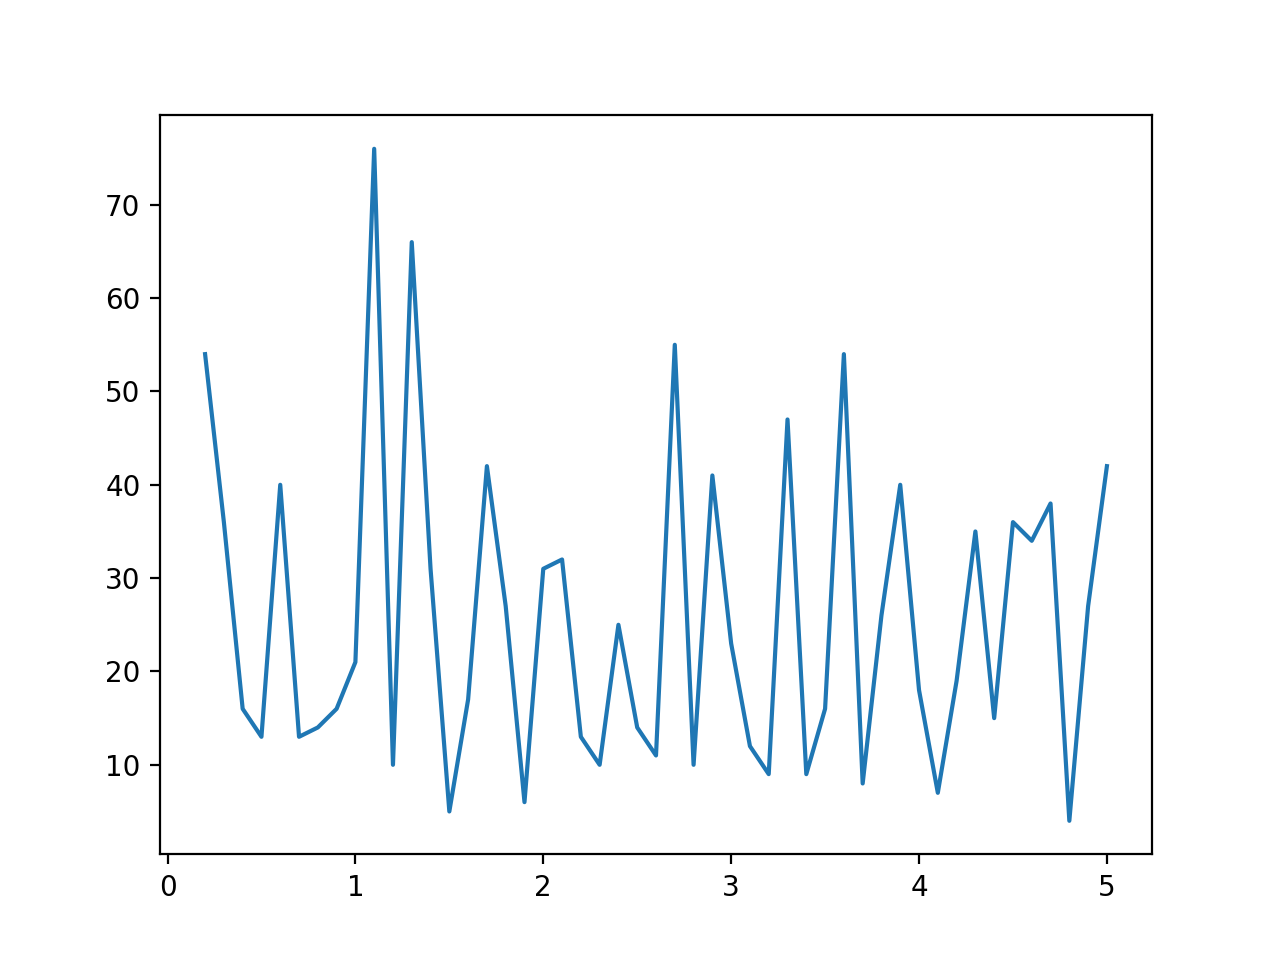
\includegraphics[width=\textwidth]{32maybe2.png}

Convergence of the PLA is not really dependent on the separation so much as the magnitude of
$\vec{x_n} \in X$. So it is unsurprising that there is little variation in the number of 
iterations required for convergence. This test would be better if it was done for each sep value
several times, but it is evident nonetheless that there is not much difference in each sep, save
for the small separations, which are slightly larger in value.


\subsection*{Problem 3.8}

\textit{Show that among all hypotheses, the one that minimizes the least squares $E_{out}$ is}

$$h^*(x) = \mathbb{E}[y | x]$$

We can rewrite the error function and expand from there as follows:

\begin{align*}
  E_{out}(h) &= \mathbb{E}[(h(\vec{x}) - y)^2] \\
  &= \mathbb{E}[((h(\vec{x}) - \mathbb{E}[y|\vec{x}]) + (\mathbb{E}[y|\vec{x}] - y))^2] \\
  &= \mathbb{E}[(h(\vec{x})-\mathbb{E}[y|\vec{x}])^2 + 2(h(\vec{x}) - \mathbb{E}[y|\vec{x}])(\mathbb{E}[y|\vec{x}] - y) + (\mathbb{E}[y|\vec{x}] - y)^2] \\ 
\end{align*}

Now, $\mathbb{E}[2(h(\vec{x}) - \mathbb{E}[y|\vec{x}])(\mathbb{E}[y|\vec{x}] - y)] = 0$ and $\mathbb{E}[(\mathbb{E}[y|\vec{x}] - y)^2] = 0$, so we finally have

$$E_{out}(h) = \mathbb{E}[(h(\vec{x}) - \mathbb{E}[y|\vec{x}])^2]$$

Which is obviously minimized when $h(\vec{x}) = \mathbb{E}[y|\vec{x}]$ since in this case 
$E_{out} = 0$, the answer we
desired for $h^*(\vec{x})$.

Now, we can write $y$ as $y = h^*(\vec{x}) + \epsilon(\vec{x})$ which can be rewritten as

$$y = \mathbb{E}[y|\vec{x}] + \epsilon(\vec{x}).$$

So in order to keep our desired $E_{out}$, we must have $\mathbb{E}[\epsilon(\vec{x})] = 0$.

\subsection*{Handwritten Digits Data}

\textit{}

\begin{enumerate}[(a)]
  \item \textit{Plot two of the digit images}

    \begin{center}
    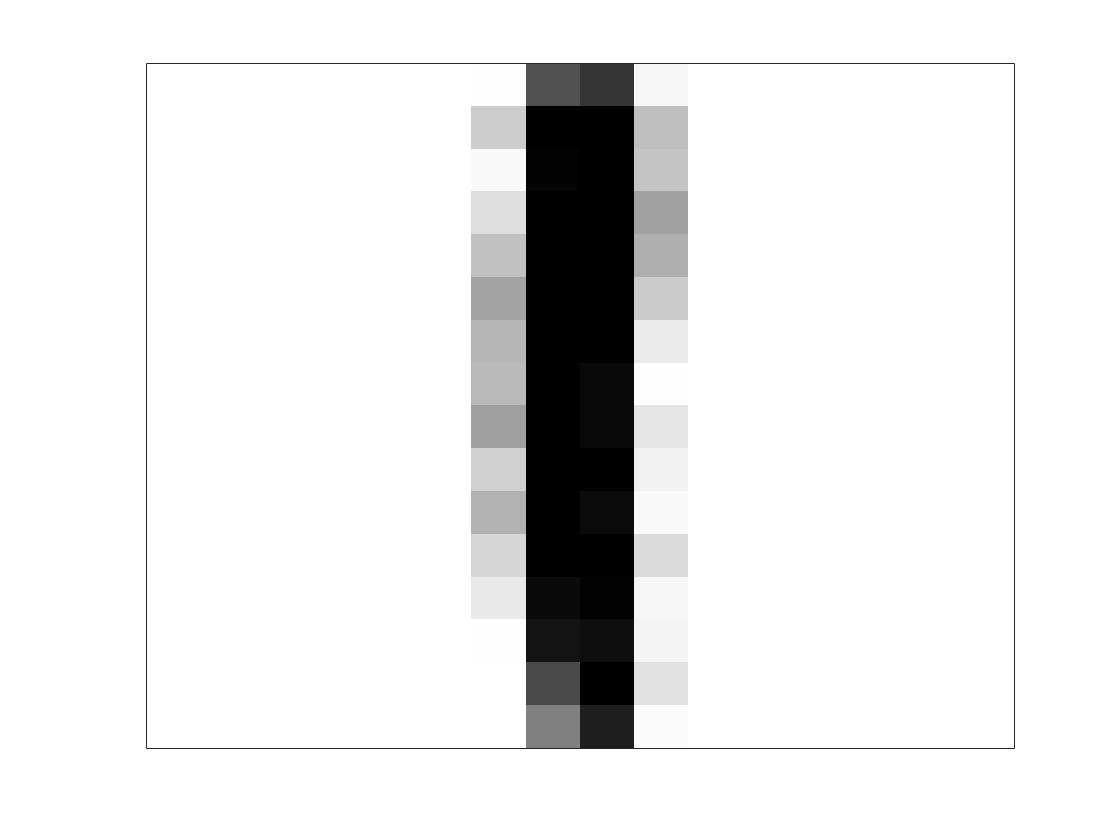
\includegraphics[width=.4\textwidth]{im1.jpg}
    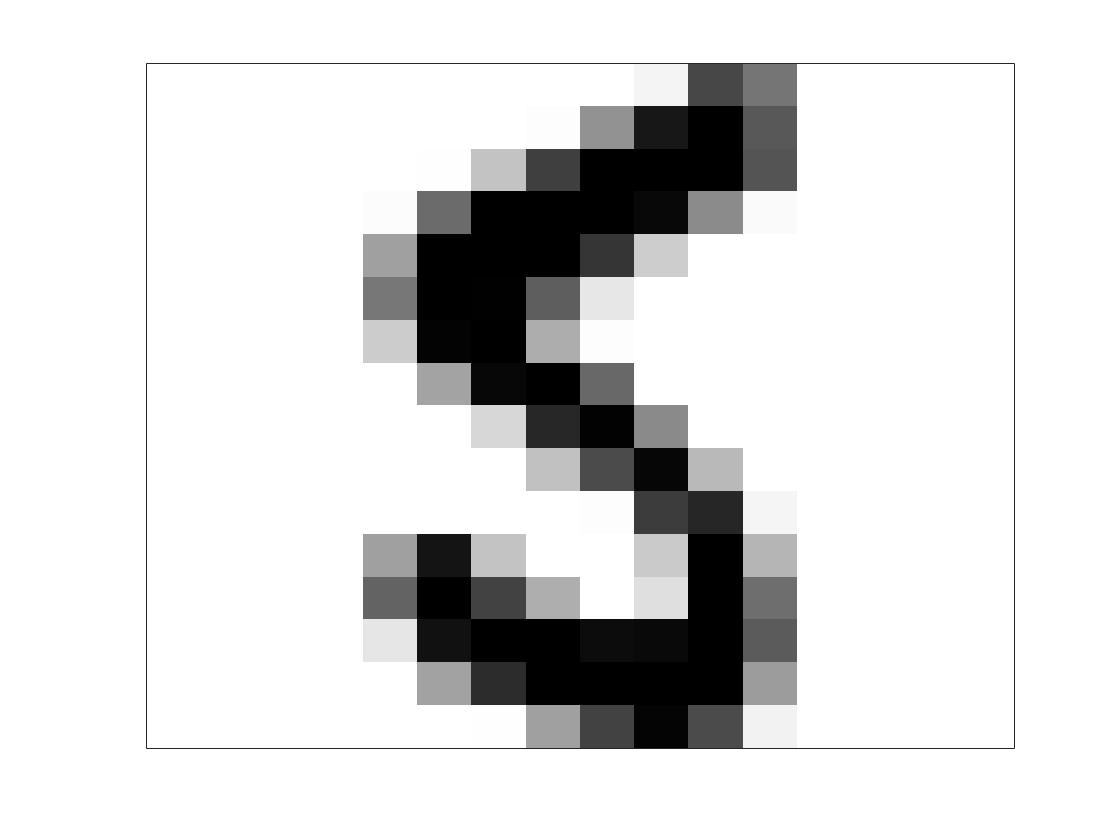
\includegraphics[width=.4\textwidth]{im5.jpg}
    \end{center}

  \item \textit{Develop two features to measure properties of teh image that would be useful in
    distinguishing between 1 and 5, e.g. symmetry and average intensity. Give the mathematical
    definition of the two features.}

    Average intensity and symmetry over the center vertical axis will be the two features used.

    Average intensity is given by the average value of 256 pixels. Defining pixels as $p_i$ for 
    $i = 0, \dots, 255$, we have for the definition

    $$Intensity = \frac{1}{256} \sum_{i=0}^{255} p_i$$

    For symmetry we will instead define the digit image as a $16\times16$ matrix $P_{16\times16}$
    where the rows of the matrix correspond to the pixel values of the rows of the image. Thus, we
    can define the reflection symmetry as an average after subtracting the right half of the image
    from the left half:

    $$Symmetry = \frac{1}{128} \sum_{i=0,j=0}^{i=15,j=7} (P_{ij} - P_{i,15-j})$$

  \item \textit{As in the text, give a 2D scatter plot of the features. For each data example,
    plot the two features with a red 'x' if it is a 5 and a blue 'o' if it is a 1.}

    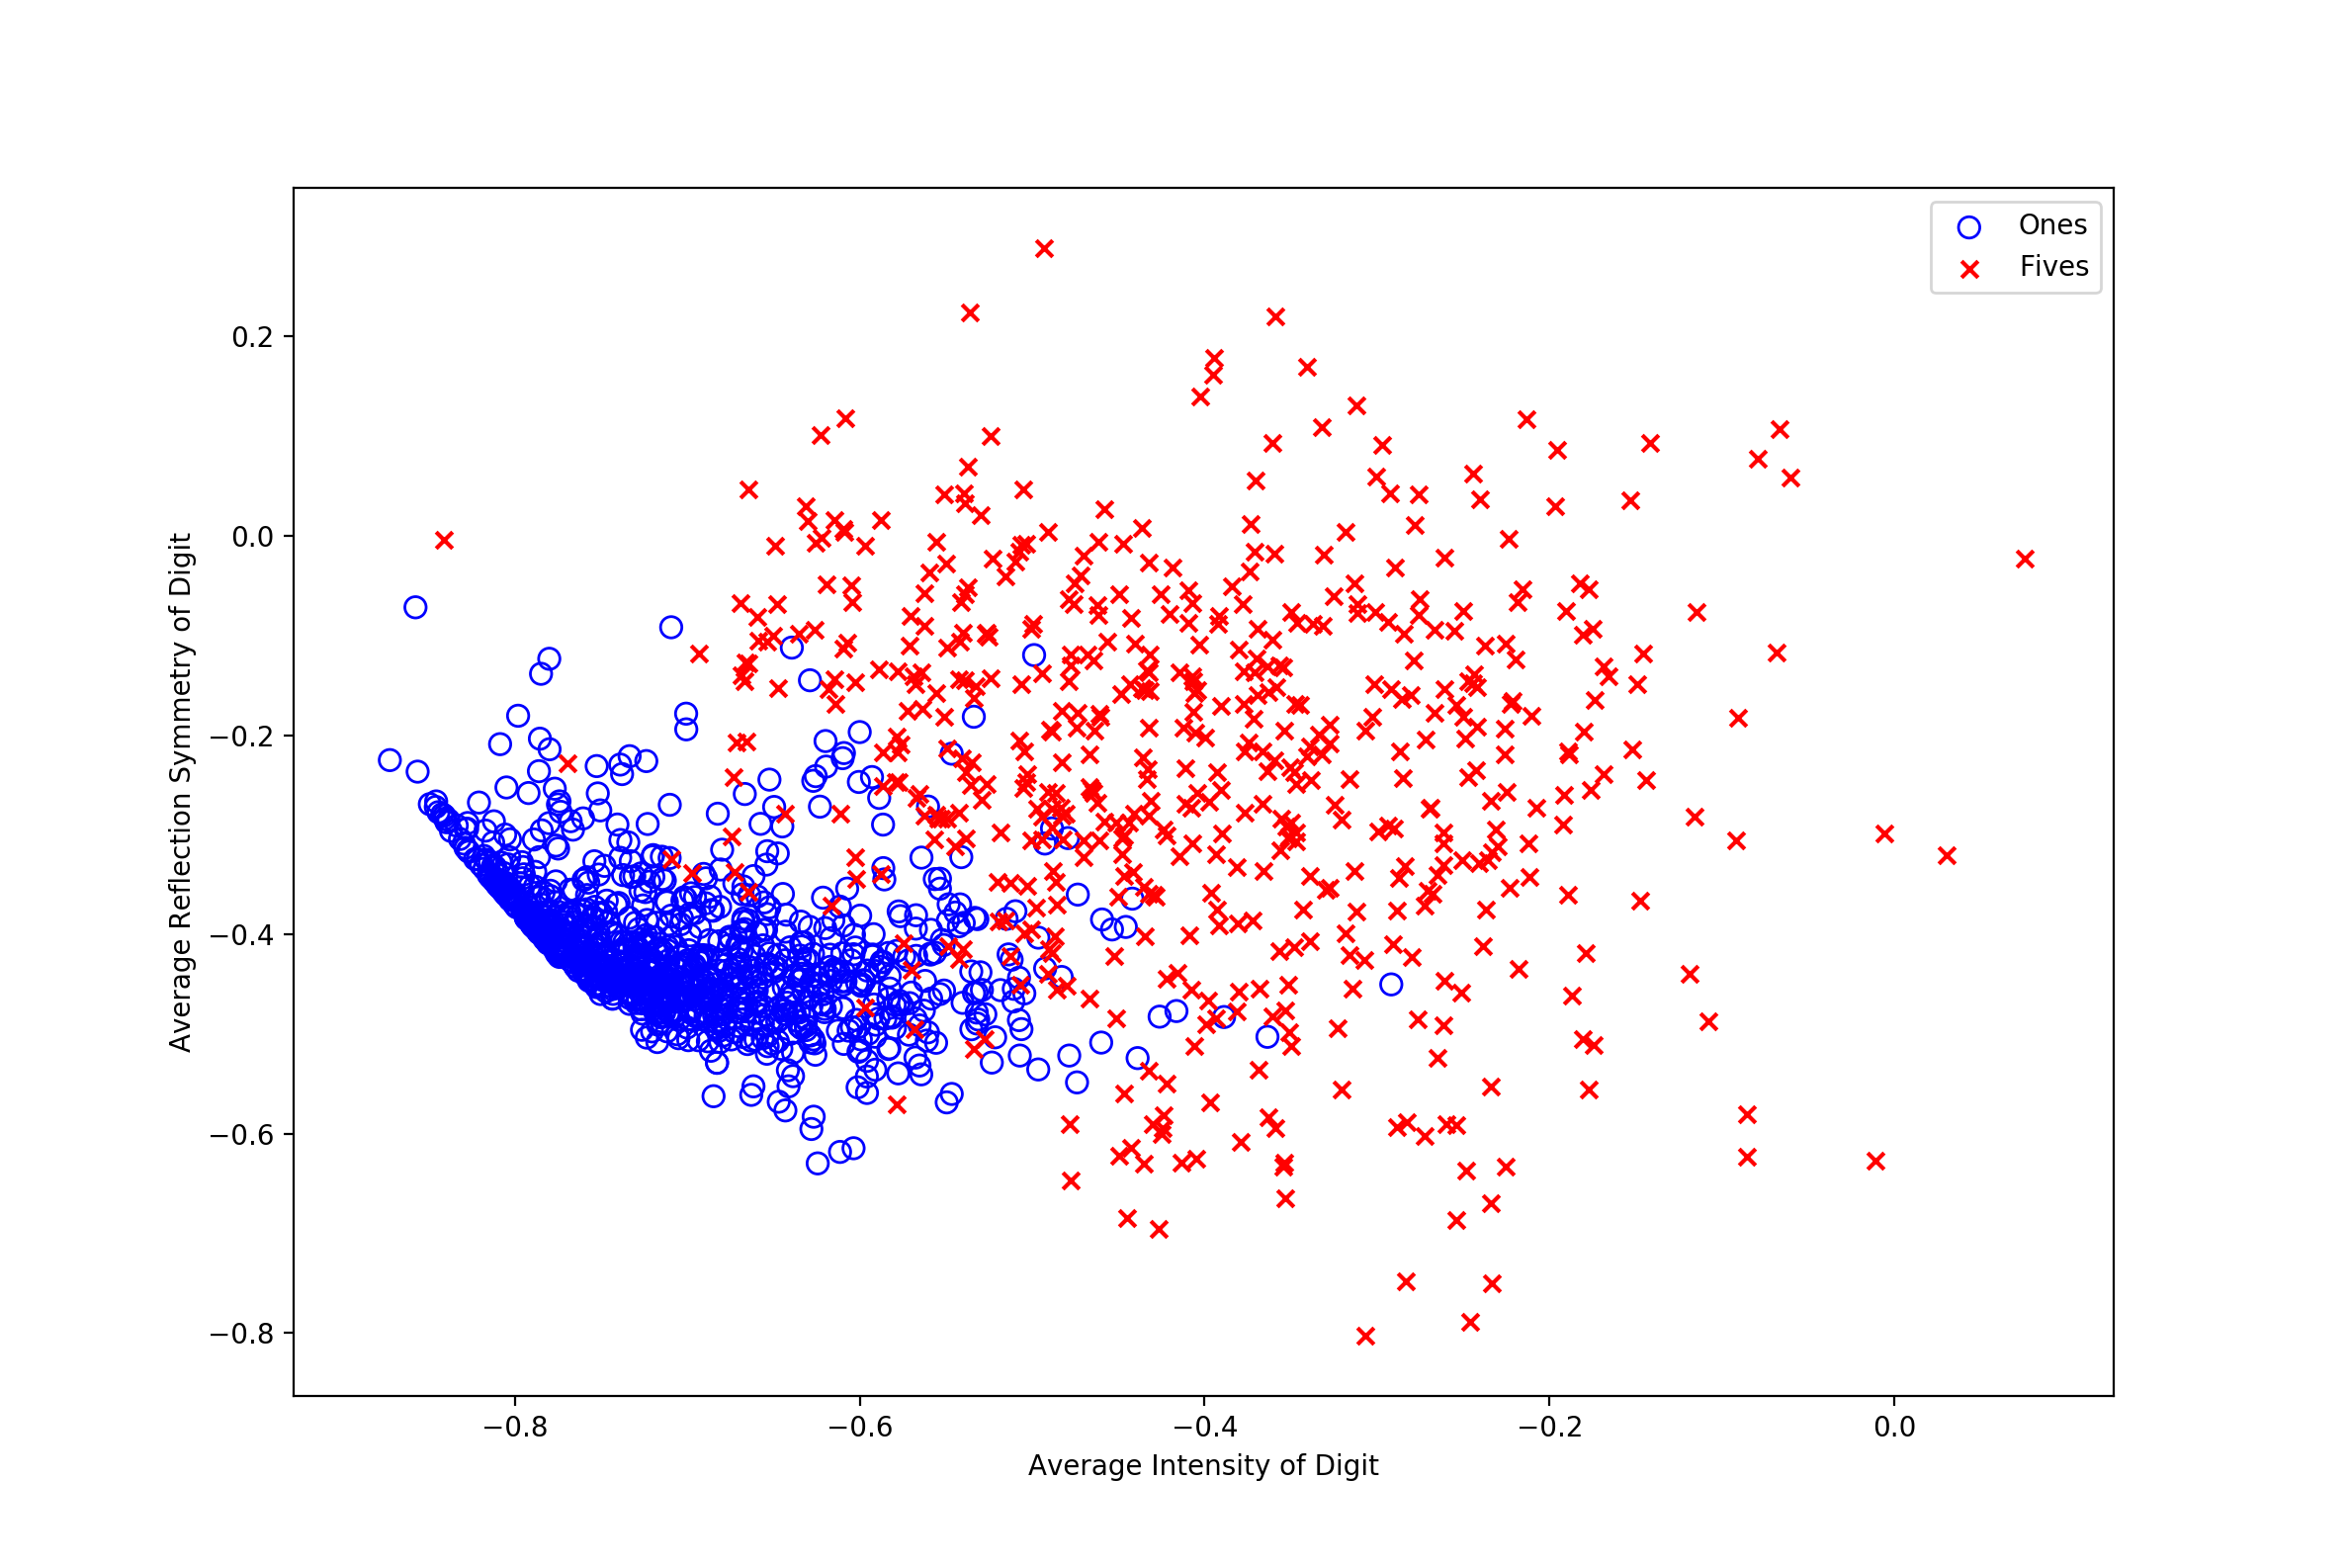
\includegraphics[width=\textwidth]{handwrittenfeatures.png}

\end{enumerate}





\end{document}
